\documentclass[11pt, aspectratio=169]{beamer}
\usetheme{copenhagen}
\usecolortheme{beaver}
\setbeamertemplate{navigation symbols}{}
\usepackage[utf8]{inputenc}
\usepackage{subcaption}
\usepackage{graphicx}
\usepackage{array}
\usepackage{longtable}
\usepackage{quotes}
\usepackage{amsmath}
\usepackage{hyperref}

\title{Uncertainty quantification in Bayesian Neural Networks using cubature rules}
\author{Qazi Zarif Ul Islam}
\date{April 26}

\begin{document}
\maketitle

\begin{frame}
    \begin{figure}
        \centering
        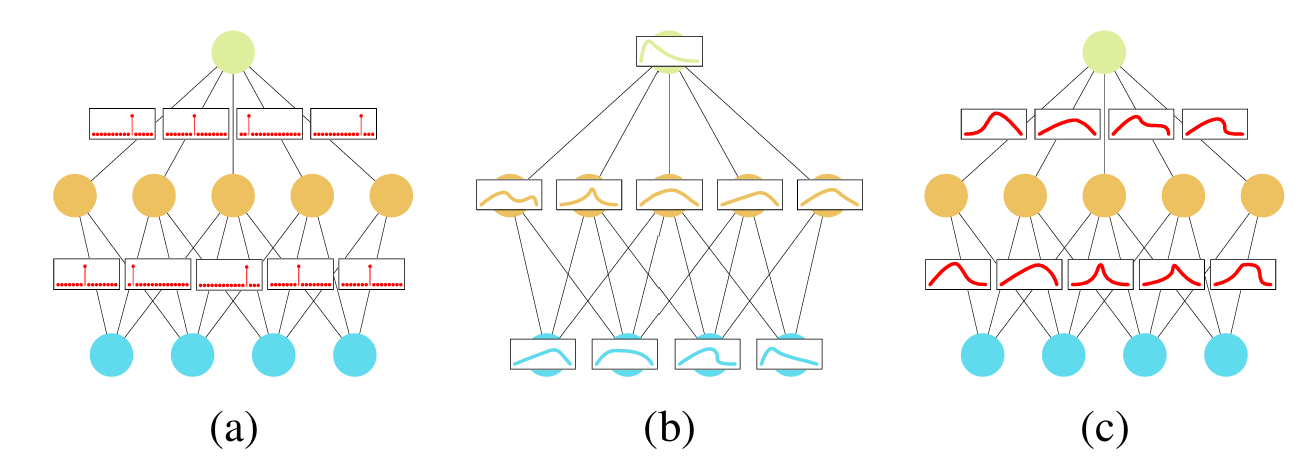
\includegraphics[width=0.8\textwidth]{figs/BNN.png}
    \end{figure}
\end{frame}

\begin{frame}{Bayesian Neural Networks}
    \underline{What is a Bayesian Neural Network?}

    A \textbf<overlay specification>{Bayesian Neural Network} is a neural networks
    where the learnable parameters \textbf{$\theta_i$ are probability distributions}
    instead of scalars.

    e.g. the weights could be Normal distributed like so,
    \begin{align}
        w_i = \mathcal{N}(\mu_i, \sigma_i^2)
    \end{align}

    - The activation functions could be stochastic too!

    - \textbf{Ensemble learning} takes place in a BNN by letting the model 
    train with multiple distributions of the learnable parameters $\theta$



\end{frame}

\begin{frame}
    \underline{How does it work?}

    \begin{itemize}
        \item Choose a \textbf{Stochastic model} i.e.  prior distributions for $p(\mathbf{\theta})$ and $p(\mathbf{y|x,\boldsymbol{\theta}})$
        \item Obtain the posterior probability
            \begin{equation}
                p(\boldsymbol{\theta}|D) = \frac{p(D_y|D_x,\boldsymbol{\theta})p(\boldsymbol{\theta})}{\int_\theta p(D_y|D_x, \boldsymbol{\theta'})p(\boldsymbol{\theta'})d\boldsymbol{\theta'}}
            \end{equation}

            where, \\
                $D_y$ = Data labels \\ 
                $D_x$ = Data inputs \\

        \item Computing the integral, $\int_\theta p(D_y|D_x, \boldsymbol{\theta'})p(\boldsymbol{\theta'})d\boldsymbol{\theta'}$ is very difficult. 
        \item To address this, two broad approaches are followed:
            \begin{enumerate}
                \item MCMC (Markov chain monte carlo)
                \item Variational inference
            \end{enumerate}
    \end{itemize}

\end{frame}

\begin{frame}{ Bayesian Neural Networks}
    \underline{Motivation} \\
    The main goal is to get a better idea about the \textbf{uncertainty}. 
    For example, if all the results of the models are vastly 
    different, there's more uncertainty thereby providing a way to 
    \textit{preemptively} assess \textbf{generalizability}.
    


\end{frame}


\begin{frame}{Uncertainty quantification}    
    
    Some techniques:
    \begin{itemize}
        \item Particle filtering 
        \item Variational inference
        \item Cubature rules*
        \item and so on...
    \end{itemize}


\end{frame}

\end{document}


